\begin{figure}[t]
    \centering
    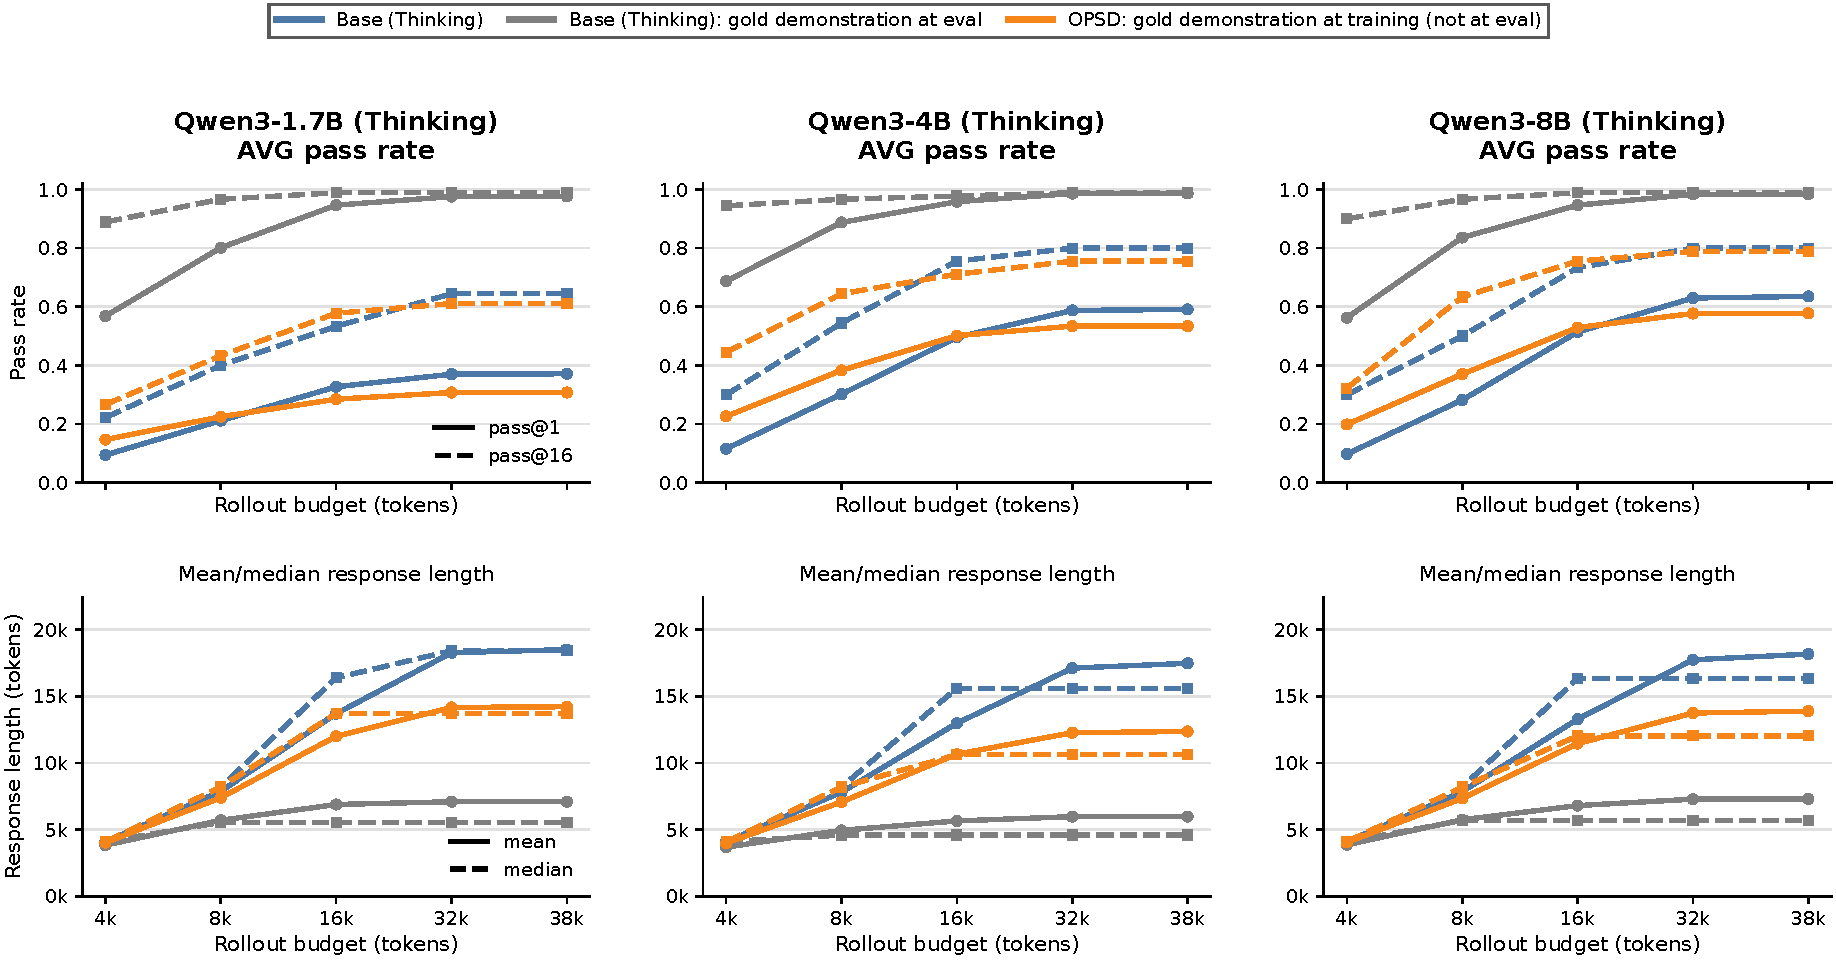
\includegraphics[width=\linewidth]{figures/avg_pass_rollout_tokens_qwen_gpt_oss_final_response_with_opsd_demo_purple_context.pdf}
    \caption{
    \textbf{\opsd{} students inherit the teacher's shorter response lengths, but not the pass@k benefits at longer rollout budgets.}
    For each Qwen3 thinking-model size (1.7B, 4B, and 8B), we compare three settings: the base model; the same base model given a gold demonstration in context, matching the setup of the \opsd{} teacher; and the \opsd{} student, evaluated without the gold demonstration in context.
    Top row: pass@1 and pass@16, averaged over AIME24, AIME25, and HMMT25.
    Bottom row: mean and median response length.
    Providing the teacher with the gold demonstration in context shortens the teacher's own rollouts without hurting pass@k, and can even improve pass@k.
    Though the \opsd{} student produces shorter responses like the teacher, the student's pass@k gains are smaller at short budgets and disappear or reverse at longer rollout budgets.
    }
    \label{fig:openthoughts_teacher_student_asymmetry}
\end{figure}
